Una vez definido y validado el pipeline de evaluación, se aplicó el protocolo anterior a los modelos entrenados. Los resultados se presentan separando los escenarios de dos y cuatro fuentes, ya que ambos problemas presentan distinta dificultad y no son directamente comparables.

En la Tabla \ref{tab:resultados-2-fuentes-sisdri} se presentan los resultados de separación en dos fuentes, mientras que en la Tabla \ref{tab:resultados-4-fuentes-sisdri} se presentan los resultados de separación en cuatro fuentes. En ambas tablas se muestran las métricas de SI-SDRi y SI-SAR, así como la desviación típica y si el modelo supera o no al \textit{baseline}.

\begin{table}[H]
    \centering
    \caption{Tabla para los resultados de separación en 2 fuentes }
    \label{tab:resultados-2-fuentes-sisdri}

    \begin{adjustbox}{center,max width=\textwidth}
        \begin{tabular}{llrrrrc}
            \toprule
            \makecell{\textbf{Función}\\\textbf{de pérdida}} &
            \textbf{Grupo} &
            \makecell{\textbf{SI-SDRi}\\\textbf{medio}} &
            \makecell{\textbf{SI-SDRi}\\\textbf{mediano}} &
            \makecell{\textbf{Desviación}\\\textbf{típica}} &
            \makecell{\textbf{SI-SAR}\\\textbf{medio}} &
            \makecell{\textbf{Supera}\\\textbf{baseline}} \\
            \midrule

            \texttt{l1}                  & principal    & -7.157  & -6.923  & 1.765 & 3.582  & No \\
            \texttt{l2}                  & principal    & -2.515  & -2.575  & 0.632 & 11.445 & No \\
            \texttt{l1\_freq}            & principal    & -7.158  & -6.924  & 1.762 & 3.578  & No \\
            \texttt{l2\_freq}            & principal    & -2.262  & -2.343  & 0.584 & 12.273 & No \\
            \texttt{logl1}               & principal    & -10.745 & -11.134 & 2.771 & -1.743 & No \\
            \texttt{logl2}               & principal    & -9.575  & -9.118  & 2.675 & 0.012  & No \\
            \texttt{log\_mag}            & principal    & -8.343  & -8.071  & 2.066 & 2.130  & No \\
            \texttt{log\_compressed\_l2} & principal    & -8.929  & -8.540  & 2.198 & 0.500  & No \\
            \texttt{lpsa}                & principal    & -9.405  & -8.905  & 2.387 & -0.303 & No \\
            \texttt{mask\_l1}            & principal    & -8.239  & -7.976  & 1.907 & 2.107  & No \\
            \texttt{l\_mrs}              & avanzado     & -9.583  & -9.591  & 2.345 & -0.192 & No \\
            \texttt{lpsa\_phase}         & avanzado     & -8.158  & -8.750  & 1.892 & -7.500 & No \\
            \texttt{deep\_feature}       & experimental & -0.091  & -0.098  & 0.063 & 22.996 & No \\
            \texttt{deep\_feature\_emd}  & experimental & -0.081  & -0.082  & 0.042 & 23.435 & No \\

            \bottomrule
        \end{tabular}
    \end{adjustbox}
\end{table}

\begin{table}[H]
    \centering
    \caption{Tabla para los resultados de separación en 4 fuentes}
    \label{tab:resultados-4-fuentes-sisdri}

    \begin{adjustbox}{center,max width=\textwidth}
        \begin{tabular}{llrrrrc}
            \toprule
            \makecell{\textbf{Función}\\\textbf{de pérdida}} &
            \textbf{Grupo} &
            \makecell{\textbf{SI-SDRi}\\\textbf{medio}} &
            \makecell{\textbf{SI-SDRi}\\\textbf{mediano}} &
            \makecell{\textbf{Desviación}\\\textbf{típica}} &
            \makecell{\textbf{SI-SAR}\\\textbf{medio}} &
            \makecell{\textbf{Supera}\\\textbf{baseline}} \\
            \midrule

            \texttt{l1}                  & principal    & -4.811 & -5.085 & 1.650 & -1.933 & No \\
            \texttt{l2}                  & principal    & -0.065 & -0.066 & 0.038 & 20.263 & No \\
            \texttt{l1\_freq}            & principal    & -4.814 & -5.089 & 1.651 & -1.940 & No \\
            \texttt{l2\_freq}            & principal    & -0.069 & -0.070 & 0.037 & 20.437 & No \\
            \texttt{logl1}               & principal    & -9.356 & -9.176 & 2.587 & -8.803 & No \\
            \texttt{logl2}               & principal    & -5.231 & -5.183 & 1.850 & -2.760 & No \\
            \texttt{log\_mag}            & principal    & -6.767 & -6.589 & 2.151 & -4.835 & No \\
            \texttt{log\_compressed\_l2} & principal    & -6.801 & -6.708 & 1.946 & -5.555 & No \\
            \texttt{lpsa}                & principal    & --     & --     & --    & --     & -- \\
            \texttt{mask\_l1}            & principal    & -6.424 & -6.297 & 2.025 & -4.469 & No \\
            \texttt{l\_mrs}              & avanzado     & -7.391 & -7.198 & 2.059 & -6.082 & No \\
            \texttt{lpsa\_phase}         & avanzado     & -1.042 & -1.213 & 0.776 & -1.671 & No \\
            \texttt{deep\_feature}       & experimental & -0.018 & -0.020 & 0.055 & 16.532 & No \\
            \texttt{deep\_feature\_emd}  & experimental & 0.006  & 0.004  & 0.059 & 17.562 & Sí \\

            \bottomrule
        \end{tabular}
    \end{adjustbox}
\end{table}

\subsubsection{Rankings}

En esta sección se presentan los rankings de los modelos entrenados, ordenados por la métrica de SI-SDR medio, para los escenarios de dos y cuatro fuentes. Estos rankings permiten identificar rápidamente qué modelos han obtenido un mejor rendimiento en términos de separación de fuentes.
\begin{table}[H]
\centering
\caption{Ranking para los resultados de separación en 2 fuentes}
\label{tab:ranking-2-fuentes}


\begin{adjustbox}{center,max width=\textwidth}
    \begin{tabular}{clrrrrc}
        \toprule
        \makecell{\textbf{Rank}} &
        \makecell{\textbf{Función}\\\textbf{de pérdida}} &
        \makecell{\textbf{SI-SDR}\\\textbf{medio}} &
        \makecell{\textbf{SI-SDR}\\\textbf{mediano}} &
        \makecell{\textbf{SI-SDR}\\\textbf{desviación típica}} &
        \makecell{\textbf{SI-SAR}\\\textbf{medio}} &
        \makecell{\textbf{Supera}\\\textbf{baseline}} \\
        \midrule

        1 & deep\_feature\_emd & -0.099 & -0.109 & 0.063 & 23.435 & No \\
        2 & deep\_feature & -0.109 & -0.104 & 0.091 & 22.996 & No \\
        3 & l2\_freq & -2.281 & -2.349 & 0.563 & 12.273 & No \\
        4 & l2 & -2.533 & -2.622 & 0.608 & 11.445 & No \\
        5 & l1 & -7.175 & -6.975 & 1.737 & 3.582 & No \\
        6 & l1\_freq & -7.176 & -6.976 & 1.734 & 3.578 & No \\
        7 & lpsa\_phase & -8.176 & -8.721 & 1.915 & -7.500 & No \\
        8 & mask\_l1 & -8.257 & -8.027 & 1.871 & 2.107 & No \\
        9 & log\_mag & -8.361 & -8.123 & 2.033 & 2.130 & No \\
        10 & log\_compressed\_l2 & -8.947 & -8.556 & 2.164 & 0.500 & No \\
        11 & lpsa & -9.423 & -8.957 & 2.353 & -0.303 & No \\
        12 & logl2 & -9.593 & -9.140 & 2.642 & 0.012 & No \\
        13 & l\_mrs & -9.602 & -9.638 & 2.314 & -0.193 & No \\
        14 & logl1 & -10.763 & -11.084 & 2.740 & -1.743 & No \\

        \bottomrule
    \end{tabular}
\end{adjustbox}


\end{table}

\begin{table}[H]
\centering
\caption{Ranking para los resultados de separación en 4 fuentes}
\label{tab:ranking-4-fuentes}


\begin{adjustbox}{center,max width=\textwidth}
    \begin{tabular}{clrrrrc}
        \toprule
        \makecell{\textbf{Rank}} &
        \makecell{\textbf{Función}\\\textbf{de pérdida}} &
        \makecell{\textbf{SI-SDR}\\\textbf{medio}} &
        \makecell{\textbf{SI-SDR}\\\textbf{mediano}} &
        \makecell{\textbf{SI-SDR}\\\textbf{desviación típica}} &
        \makecell{\textbf{SI-SAR}\\\textbf{medio}} &
        \makecell{\textbf{Supera}\\\textbf{baseline}} \\
        \midrule

        1 & deep\_feature\_emd & -0.099 & -0.109 & 0.063 & 23.435 & No \\
        2 & deep\_feature & -0.109 & -0.104 & 0.091 & 22.996 & No \\
        3 & l2\_freq & -2.281 & -2.349 & 0.563 & 12.273 & No \\
        4 & l2 & -2.533 & -2.622 & 0.608 & 11.445 & No \\
        5 & l1 & -7.175 & -6.975 & 1.737 & 3.582 & No \\
        6 & l1\_freq & -7.176 & -6.976 & 1.734 & 3.578 & No \\
        7 & lpsa\_phase & -8.176 & -8.721 & 1.915 & -7.500 & No \\
        8 & mask\_l1 & -8.257 & -8.027 & 1.871 & 2.107 & No \\
        9 & log\_mag & -8.361 & -8.123 & 2.033 & 2.130 & No \\
        10 & log\_compressed\_l2 & -8.947 & -8.556 & 2.164 & 0.500 & No \\
        11 & lpsa & -9.423 & -8.957 & 2.353 & -0.303 & No \\
        12 & logl2 & -9.593 & -9.140 & 2.642 & 0.012 & No \\
        13 & l\_mrs & -9.602 & -9.638 & 2.314 & -0.193 & No \\
        14 & logl1 & -10.763 & -11.084 & 2.740 & -1.743 & No \\

        \bottomrule
    \end{tabular}
\end{adjustbox}


\end{table}

\subsubsection{Gráficos de barras}

Se han generado dos gráficos de barras para dar una imagen que represente visualmente los resultados:

\begin{figure}[H]
    \centering
    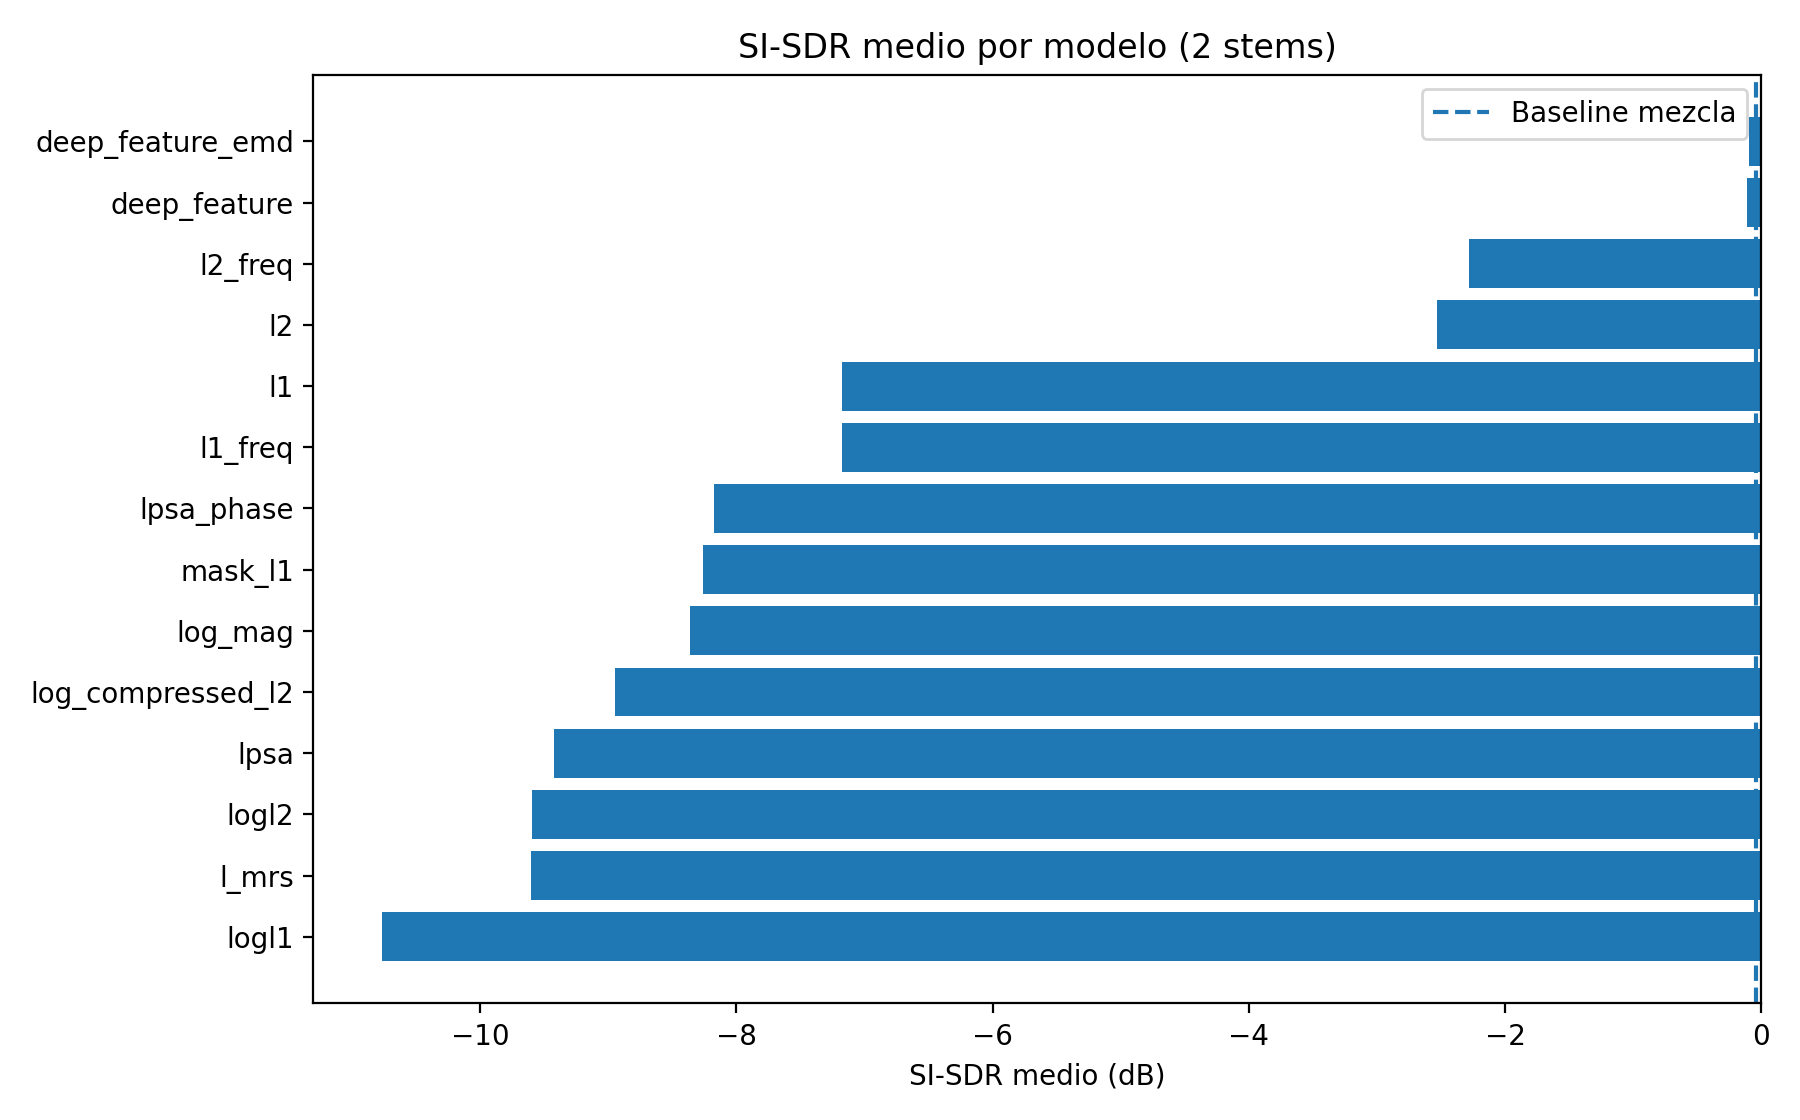
\includegraphics[width=\textwidth,keepaspectratio]{commons/barplot_sisdr_2stems.png}
    \caption{Gráfico de barras de los valores SI-SDR de cada función de pérdida en la separación de dos fuentes}
    \label{fig:barplot-2sources}
\end{figure}

\begin{figure}[H]
    \centering
    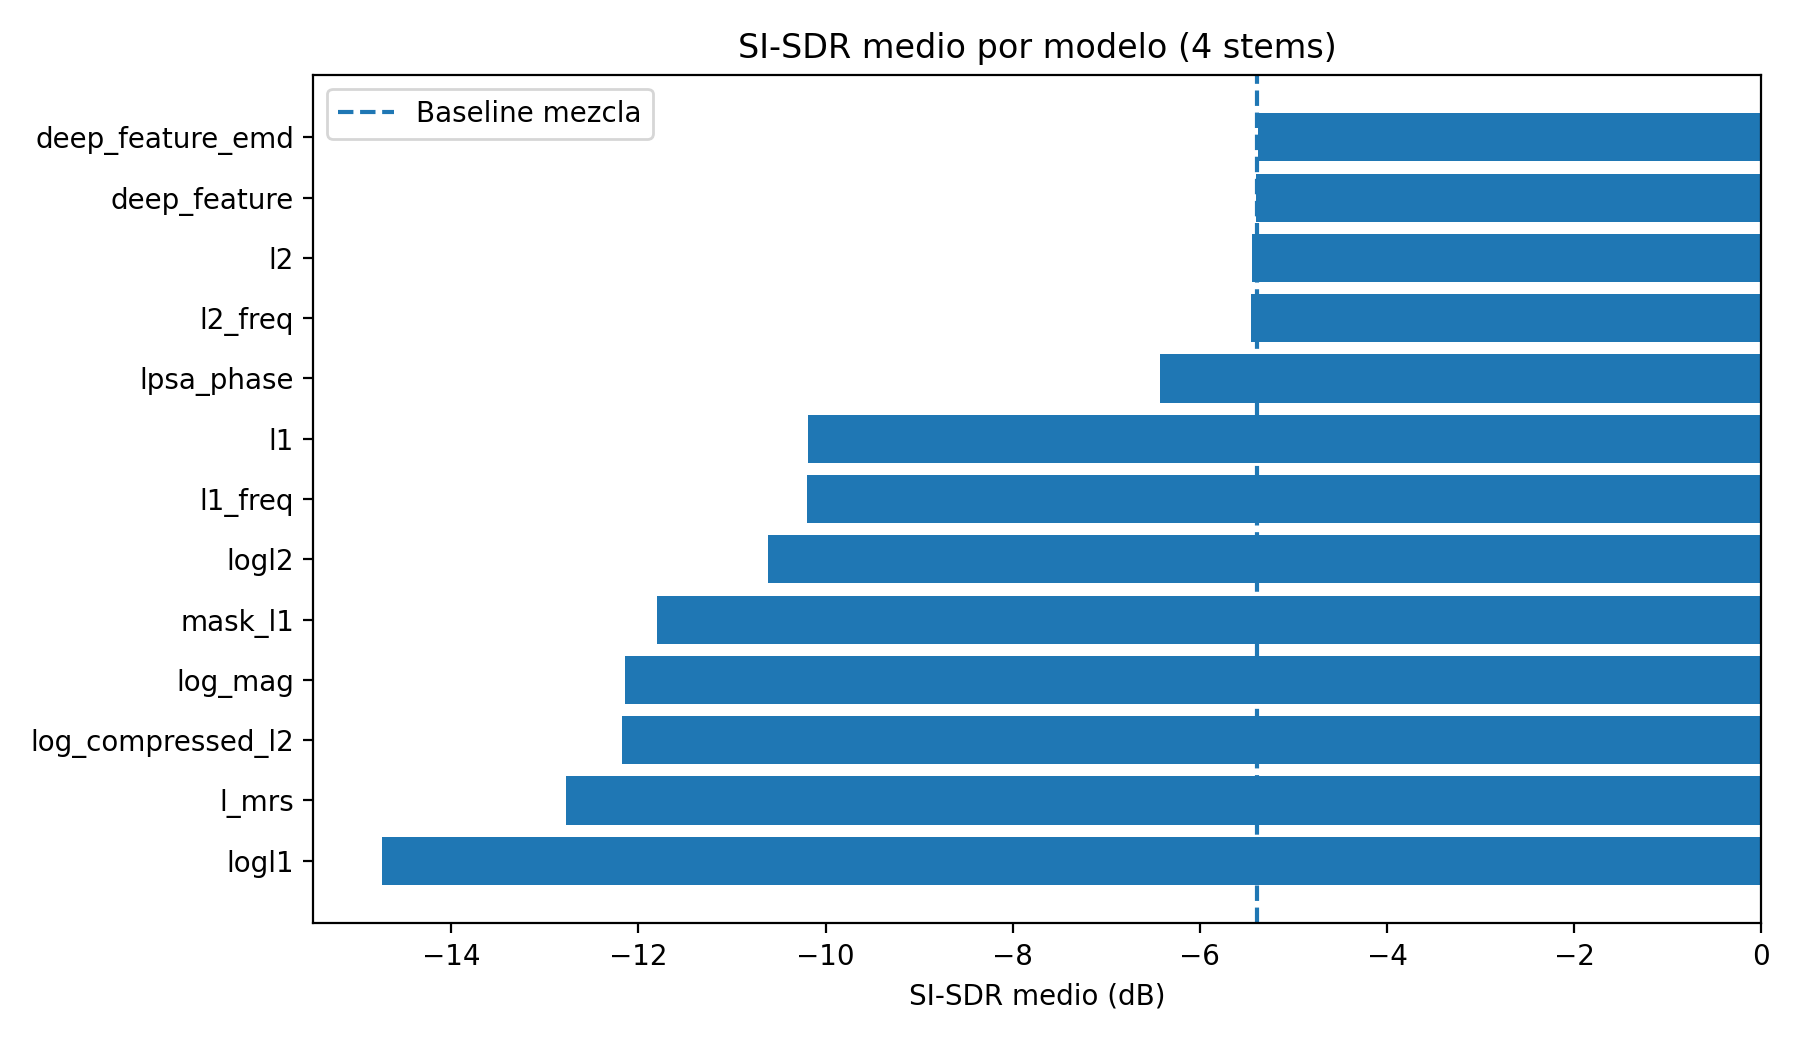
\includegraphics[width=\textwidth,keepaspectratio]{commons/barplot_sisdr_4stems.png}
    \caption{Gráfico de barras de los valores SI-SDR de cada función de pérdida en la separación de cuatro fuentes}
    \label{fig:barplot-4sources}
\end{figure}



